\documentclass[a4paper, 12pt]{article}

% packages
\usepackage{amssymb}
\usepackage[fleqn]{mathtools}
\usepackage{tikz}
\usepackage{enumerate}
\usepackage{bussproofs}
\usepackage{xcolor}
\usepackage[margin=1.3cm]{geometry}
\usepackage{logicproof}
\usepackage{diagbox}
\usepackage{listings}
\usepackage{graphicx}
\usepackage{lstautogobble}
\usepackage{hyperref}
\usepackage{multirow}
\usepackage{tipa}
\usepackage{pgfplots}
\usepackage{adjustbox}

% tikz libraries
\usetikzlibrary{
    decorations.pathreplacing,
    arrows,
    shapes.gates.logic.US,
    circuits.logic.US,
    calc,
    automata,
    positioning,
    intersections
}

\pgfplotsset{compat=1.16}

\pgfmathdeclarefunction{gauss}{2}{%
  \pgfmathparse{1/(#2*sqrt(2*pi))*exp(-((x-#1)^2)/(2*#2^2))}%
}

\allowdisplaybreaks % allow environments to break
\setlength\parindent{0pt} % no indent

% shorthand for verbatim
% this clashes with logicproof, so maybe fix this at some point?
\catcode`~=\active
\def~#1~{\texttt{#1}}

% code listing
\lstdefinestyle{main}{
    numberstyle=\tiny,
    breaklines=true,
    showspaces=false,
    showstringspaces=false,
    tabsize=2,
    numbers=left,
    basicstyle=\ttfamily,
    columns=fixed,
    fontadjust=true,
    basewidth=0.5em,
    autogobble,
    xleftmargin=3.0ex,
    mathescape=true
}
\newcommand{\dollar}{\mbox{\textdollar}} %
\lstset{style=main}

% augmented matrix
\makeatletter
\renewcommand*\env@matrix[1][*\c@MaxMatrixCols c]{%
\hskip -\arraycolsep
\let\@ifnextchar\new@ifnextchar
\array{#1}}
\makeatother

% ceiling / floor
\DeclarePairedDelimiter{\ceil}{\lceil}{\rceil}
\DeclarePairedDelimiter{\floor}{\lfloor}{\rfloor}

% custom commands
\newcommand{\indefint}[2]{\int #1 \, \mathrm{d}#2}
\newcommand{\defint}[4]{\int_{#1}^{#2} #3 \, \mathrm{d}#4}
\newcommand{\pdif}[2]{\frac{\partial #1}{\partial #2}}
\newcommand{\dif}[2]{\frac{\mathrm{d}#1}{\mathrm{d}#2}}
\newcommand{\limit}[2]{\raisebox{0.5ex}{\scalebox{0.8}{$\displaystyle{\lim_{#1 \to #2}}$}}}
\newcommand{\limitsup}[2]{\raisebox{0.5ex}{\scalebox{0.8}{$\displaystyle{\limsup_{#1 \to #2}}$}}}
\newcommand{\summation}[2]{\sum\limits_{#1}^{#2}}
\newcommand{\product}[2]{\prod\limits_{#1}^{#2}}
\newcommand{\intbracket}[3]{\left[#3\right]_{#1}^{#2}}
\newcommand{\laplace}{\mathcal{L}}
\newcommand{\fourier}{\mathcal{F}}
\newcommand{\mat}[1]{\boldsymbol{#1}}
\renewcommand{\vec}[1]{\boldsymbol{#1}}
\newcommand{\rowt}[1]{\begin{bmatrix}
    #1
\end{bmatrix}^\top}
\DeclareMathOperator*{\argmax}{argmax}
\DeclareMathOperator*{\argmin}{argmin}

\newcommand{\lto}[0]{\leadsto\ }

\newcommand{\ulsmash}[1]{\underline{\smash{#1}}}

\newcommand{\powerset}[0]{\wp}
\renewcommand{\emptyset}[0]{\varnothing}

\makeatletter
\newsavebox{\@brx}
\newcommand{\llangle}[1][]{\savebox{\@brx}{\(\m@th{#1\langle}\)}%
  \mathopen{\copy\@brx\kern-0.5\wd\@brx\usebox{\@brx}}}
\newcommand{\rrangle}[1][]{\savebox{\@brx}{\(\m@th{#1\rangle}\)}%
  \mathclose{\copy\@brx\kern-0.5\wd\@brx\usebox{\@brx}}}
\makeatother
\newcommand{\lla}{\llangle}
\newcommand{\rra}{\rrangle}
\newcommand{\la}{\langle}
\newcommand{\ra}{\rangle}
\newcommand{\crnr}[1]{\text{\textopencorner} #1 \text{\textcorner}}
\newcommand{\bnfsep}[0]{\ |\ }
\newcommand{\concsep}[0]{\ ||\ }

\newcommand{\axiom}[1]{\AxiomC{#1}}
\newcommand{\unary}[1]{\UnaryInfC{#1}}
\newcommand{\binary}[1]{\BinaryInfC{#1}}
\newcommand{\trinary}[1]{\TrinaryInfC{#1}}
\newcommand{\quaternary}[1]{\QuaternaryInfC{#1}}
\newcommand{\quinary}[1]{\QuinaryInfC{#1}}
\newcommand{\dproof}[0]{\DisplayProof}
\newcommand{\llabel}[1]{\LeftLabel{\scriptsize #1}}
\newcommand{\rlabel}[1]{\RightLabel{\scriptsize #1}}

\newcommand{\ttbs}{\char`\\}
\newcommand{\lrbt}[0]{\ \bullet\ }

% colours
\newcommand{\violet}[1]{\textcolor{violet}{#1}}
\newcommand{\blue}[1]{\textcolor{blue}{#1}}
\newcommand{\red}[1]{\textcolor{red}{#1}}
\newcommand{\teal}[1]{\textcolor{teal}{#1}}

% reasoning proofs
\usepackage{ltablex}
\usepackage{environ}
\keepXColumns
\NewEnviron{reasoning}{
    \begin{tabularx}{\textwidth}{rlX}
        \BODY
    \end{tabularx}
}
\newcommand{\proofline}[3]{$(#1)$ & $#2$ & \hfill #3 \smallskip \\}
\newcommand{\proofarbitrary}[1]{& take arbitrary $#1$ \smallskip \\}
\newcommand{\prooftext}[1]{\multicolumn{3}{l}{#1} \smallskip \\}
\newcommand{\proofmath}[3]{$#1$ & = $#2$ & \hfill #3 \smallskip \\}
\newcommand{\prooftherefore}[1]{& $\therefore #1$ \smallskip \\}
\newcommand{\proofbc}[0]{\prooftext{\textbf{Base Case}}}
\newcommand{\proofis}[0]{\prooftext{\textbf{Inductive Step}}}

% ER diagrams
\newcommand{\nattribute}[4]{
    \node[draw, state, inner sep=0cm, minimum size=0.2cm, label=#3:{#4}] (#1) at (#2) {};
}
\newcommand{\mattribute}[4]{
    \node[draw, state, accepting, inner sep=0cm, minimum size=0.2cm, label=#3:{#4}] (#1) at (#2) {};
}
\newcommand{\dattribute}[4]{
    \node[draw, state, dashed, inner sep=0cm, minimum size=0.2cm, label=#3:{#4}] (#1) at (#2) {};
}
\newcommand{\entity}[3]{
    \node[] (#1-c) at (#2) {#3};
    \node[inner sep=0cm] (#1-l) at ($(#1-c) + (-1, 0)$) {};
    \node[inner sep=0cm] (#1-r) at ($(#1-c) + (1, 0)$) {};
    \node[inner sep=0cm] (#1-u) at ($(#1-c) + (0, 0.5)$) {};
    \node[inner sep=0cm] (#1-d) at ($(#1-c) + (0, -0.5)$) {};
    \draw
    ($(#1-c) + (-1, 0.5)$) -- ($(#1-c) + (1, 0.5)$) -- ($(#1-c) + (1, -0.5)$) -- ($(#1-c) + (-1, -0.5)$) -- cycle;
}
\newcommand{\relationship}[3]{
    \node[] (#1-c) at (#2) {#3};
    \node[inner sep=0cm] (#1-l) at ($(#1-c) + (-1, 0)$) {};
    \node[inner sep=0cm] (#1-r) at ($(#1-c) + (1, 0)$) {};
    \node[inner sep=0cm] (#1-u) at ($(#1-c) + (0, 1)$) {};
    \node[inner sep=0cm] (#1-d) at ($(#1-c) + (0, -1)$) {};
    \draw
    ($(#1-c) + (-1, 0)$) -- ($(#1-c) + (0, 1)$) -- ($(#1-c) + (1, 0)$) -- ($(#1-c) + (0, -1)$) -- cycle;
}

% AVL Trees
\newcommand{\avltri}[4]{
    \draw ($(#1)$) -- ($(#1) + #4*(0.5, -1)$) -- ($(#1) + #4*(-0.5, -1)$) -- cycle;
    \node at ($(#1) + #4*(0, -1) + (0, 0.5)$) {#3};
    \node at ($(#1) + #4*(0, -1) + (0, -0.5)$) {#2};
}

% RB Trees
\tikzset{rbtr/.style={inner sep=2pt, circle, draw=black, fill=red}}
\tikzset{rbtb/.style={inner sep=2pt, circle, draw=black, fill=black}}

% actual document
\begin{document}
    \section*{CO211 - Operating Systems \hfill Tutorial Sheets}
        \subsection*{Tutorial 1 - Introduction}
            \begin{enumerate}[1.]
                \itemsep0em
                \item
                    The issue of resource allocation shows up in different forms in different types of operating systems.
                    List the most important resources that must be managed by an operating system in the following settings;
                    \begin{enumerate}[(a)]
                        \itemsep0em
                        \item Supercomputer
                            \medskip

                            Since this is most likely used for computation, processor time as well as memory should be carefully managed.
                        \item Workstations connected to servers via a network
                            \medskip

                            Network access and bandwidth.
                        \item Smartphone
                            \medskip

                            Energy, since it is a portable device, as well as access to hardware such as the camera, GPS, as well as connectivity (Bluetooth, mobile network, etc).
                    \end{enumerate}
                \item What is the kernel of an operating system?
                    \medskip

                    The kernel of the operating system is part of the operating system that remains in memory, executing in the privileged part of the CPU.
                \item
                    Why is the separation into a user mode and a kernel mode considered good operating system design?
                    Give an example in which the execution of a user process switches from user mode to kernel mode, and then back to user mode again.
                    \medskip

                    Any bugs executing in user space should not cause the entire system to crash, since the kernel allows for recovery.
                    If all programs were to run in kernel mode, a failure would bring down the entire system.
                    An example of this switch would be writing to disk (or any system call in general).
                \item Which of the following instructions should only be allowed in kernel mode, and why?
                    \begin{enumerate}[(a)]
                        \itemsep0em
                        \item Disable all interrupts \hfill kernel only
                            \medskip

                            If something in user were to disable interrupts, the kernel would have no way of regaining control,
                        \item Read the time of day clock \hfill user
                            \medskip

                            All user processes should be able to access the time if needed.
                        \item Change the memory map \hfill kernel only
                            \medskip

                            Managing memory should be restricted to the kernel.
                        \item Set the time of day \hfill kernel only
                            \medskip

                            Processes running in user space should not be able to change the time, as it can cause issues for other processes.
                    \end{enumerate}
                \item
                    A portable operating system is one that can be ported from one system architecture to another with little modification.
                    Explain why it is infeasible to build an operating system that is portable without any modification.
                    Describe two general parts that you can find in an operating system that has been designed to be highly portable.
                    \medskip

                    Since the operating system must interact with the hardware, it's not feasible to build an OS that can interact with every hardware configuration.
                    Device drivers (\textbf{platform specific}) allow for the operating system to interact with hardware, and this can be provided by the hardware manufacturer.
                    Another part would be an API the OS provides to programs (\textbf{platform independent}), allowing them to interact with hardware via this abstraction.
            \end{enumerate}
        \subsection*{Tutorial 2 - Processes + Threads}
            \begin{enumerate}[1.]
                \itemsep0em
                \item
                    If a multithreaded process forks, a problem occurs if the child gets copies of all the parent's threads.
                    Suppose that one of the original threads was waiting for keyboard input.
                    Now two threads are waiting for keyboard input, one in each process.
                    Does this problem ever occur in single-threaded processes?
                    \medskip

                    No, this does not happen in single-threaded processes as the entire process would be blocked when waiting for input, and therefore cannot fork.
                \item
                    What is the biggest advantage of implementing threads in user space?
                    What is the biggest disadvantage?
                    \medskip

                    The biggest advantage is that it allows the thread scheduling to be managed by the programmer, and also avoids the overhead of context switching.
                    On the other hand, the main disadvantage is that if any of the user space threads were to block (to wait for input), it would context switch to another thread.
                \item If in a multithreaded web server the only way to read from a file is the normal blocking ~read()~ system call, do you think user-level threads or kernel-level threads are being used?
                    \medskip

                    Kernel-level threads are being used, as the entire web server would block if it was done with user space threads.
                \item
                    Why would a thread ever voluntarily give up the CPU by calling ~thread\_yield()~?
                    After all, since there is no periodic clock interrupts, it may never get the CPU back.
                    \medskip

                    It is done to lower the priority of the thread in the scheduler, allowing another thread to run.
                    This allows threads to cooperate.
                \item
                    The register set is a per-thread rather than a per-process item.
                    Why?
                    After all, the machine has only one set of registers.
                    \medskip

                    When a thread is stopped, it has its own contents in a register which must be saved (and then restored transparently to the thread).
                \item
                    In a system with threads, is there one stack per thread or one stack per process when user-level threads are used?
                    What about when kernel threads are used?
                    Explain.
                    \medskip

                    Since each thread can call procedures, it must have a stack per thread in order to store local variables and calls.
                    The same can be said for kernel threads.
                \item
                    In this problem you are to compare reading a file using a single-threaded file server and a multithreaded server, running on a single CPU-machine.
                    It takes 15 ms to get a request for work, dispatch it, and do the rest of the necessary processing, assuming that the data needed are in the block cache.
                    If a disk operation is needed, as is the case one-third of the time, an additional 75 ms is required, during which time the thread sleeps.
                    For this problem, assume that thread switching time is negligible.
                    How many requests/sec can the server handle if it is single-threaded?
                    If it is multithreaded?
                    \medskip

                    Let the average time for an operation be $15 + \frac{1}{3} \cdot 75 = 40$ ms.
                    Therefore, with a single thread, it can process 25 requests/s.
                    \medskip

                    We want to calculate the probability that all threads are waiting for I/O.
                    The average blocking time per thread is 25 ms, as seen above.
                    This means that the probability that all threads are blocked is $1 - (\frac{25}{40})^n = 1 - (\frac{5}{8})^n$,
                    As such, we can calculate the number of requests per second as;
                    $$\left(1 - \left(\frac{5}{8}\right)^n\right) \cdot \frac{1000}{15}$$
                    Note $\frac{1000}{15}$ requests/sec is at full efficiency.
                \item
                    Would an algorithm that performs several independent CPU-intensive calculations concurrently (e.g. matrix multiplication) be more efficient if it used threads, or if it did not use threads?
                    Why is this a hard question to answer?
                    \medskip

                    It would be more efficient as long as the overhead for threads is negligible compared to the performance increase, and the CPU is actually able to perform the computation in parallel (multiple cores), otherwise the overhead of threads will cause it to be less efficient.
                    This is difficult to answer as it depends on the problem itself, how it is divided, as well as the system specifications.
                \item IPC mechanisms
                    \begin{enumerate}[(a)]
                        \itemsep0em
                        \item What happens when a signal is received by a process?
                            \medskip

                            Other than ~SIGKILL~ and ~SIGSTOP~, the receiving process is able to choose what it does with the signal.
                            It can either ignore it, or manually handle it.
                            Otherwise, it generally terminates the process.
                        \item
                            When two processes communicate through a pipe, the kernel allocates a buffer (of size 65536 bytes in Linux) for the pipe.
                            What happens when the process at the write-end of the pipe attempts to sen additional bytes on a full pipe?
                            \medskip

                            It cannot write, and will block until the process at the read-end reads from it, thus freeing up space.
                        \item
                            What happens when the process at the write-end of the pipe attempts to send additional bytes and the process at the read-end has already closed the file descriptor associated with the read-end of the pipe?
                            \medskip

                            The writing process will have an error returned to it.
                        \item
                            The process at the write-end of the pipe wants to transmit a linked list data structure (with one integer field, an a "next" pointer) over a pipe.
                            How can it do this?
                            \medskip

                            Since they do not share address spaces, it must be serialised in some form by the sending process, which can then be converted back into a linked list by the receiving process.
                        \item
                            When would it be better for two processes to communicate via shared memory instead of pipes?
                            What about the other way around?
                            \medskip

                            It would be better for two processes to communicate via shared memory as it is faster due to the lack of kernel intervention - it also allows for bi-directional communication.
                            On the other hand, pipes are handled by the kernel, thus synchronisation does not have to be implemented by the programmer.
                    \end{enumerate}
            \end{enumerate}
        \subsection*{Tutorial 3 - Scheduling}
            \begin{enumerate}[1.]
                \itemsep0em
                \item State which of the following are true and which false.
                    \begin{enumerate}[(a)]
                        \itemsep0em
                        \item Interactive systems generally use non-preemptive processor scheduling.
                            \medskip

                            \textbf{False}.
                            An interactive system uses preemptive scheduling - if there was a background process that was taking up too much time, the user interface would appear unresponsive.
                            A preemptive scheduler allows this process to be preempted, giving control to the process running the user interface.
                        \item Turnaround times are more predictable in preemptive than in non-preemptive systems.
                            \medskip

                            \textbf{False}.
                            In a non-preemptive system, a process will run to completion (or until it blocks).
                        \item One weakness of priority scheduling is that the system will faithfully honour the priorities, but the priorities themselves may not be meaningful.
                            \medskip

                            \textbf{True}.
                            The actual priority of a job can depend on what other processes are running at the same time.
                    \end{enumerate}
                \item
                    \begin{enumerate}[(a)]
                        \itemsep0em
                        \item Give an example showing why FCFS is not an appropriate scheduling scheme for interactive users.
                            \medskip

                            Assume that there are two tasks on a system.
                            The first task, is a large computation that happens in the background, and takes a notable amount of time (and is purely CPU bound, hence no blocking).
                            The second task is a browser.
                            Since the first task would be run first, the browser will be unresponsive to the end user, since the first task occupies the resources until it finishes.
                        \item Using the previous example, show why round-robin is a better scheme for interactive users.
                            \medskip

                            Round-robin switches between the two tasks, thus ensuring both tasks get the processor periodically.
                            As such, the browser will be able to respond (since the large task can be interrupted), and the computation can continue after the browser uses up its time quantum.
                    \end{enumerate}
                \item
                    Five jobs are waiting to be run.
                    Their expected run times are $9, 6, 3, 5, X$.
                    In what order should they be run to minimise average turnaround time?
                    \medskip

                    It should be run with the shortest job first, and the longest job last ($X$ should be placed in the list $3, 5, 6, 9$ accordingly).
                \item
                    Five batch jobs, $A$ through $E$, arrive at a computer centre at essentially the same time.
                    Their estimated running times, and priorities (lower value is higher priority) are as follows;
                    \begin{center}
                        \begin{tabular}{c|c|c}
                            job & running time (minutes) & priority \\
                            \hline
                            $A$ & 15 & 6 \\
                            $B$ & 9 & 3 \\
                            $C$ & 3 & 7 \\
                            $D$ & 6 & 9 \\
                            $E$ & 12 & 4
                        \end{tabular}
                    \end{center}
                    For each of the following scheduling algorithms, determine the turnaround time for each job, and the average turnaround time for all jobs.
                    Ignore process switching overhead and assume all jobs are completely CPU bound.
                    \begin{enumerate}[(a)]
                        \itemsep0em
                        \item non-preemptive priority scheduling
                            \begin{center}
                                \begin{tabular}{c|c}
                                    job & turnaround time (minutes) \\
                                    \hline
                                    $B$ & $9$ \\
                                    $E$ & $9 + 12 = 21$ \\
                                    $A$ & $21 + 15 = 36$ \\
                                    $C$ & $36 + 3 = 39$ \\
                                    $D$ & $39 + 6 = 45$
                                \end{tabular}
                            \end{center}
                            Hence the average turnaround time is $30$ minutes.
                        \item FCFS (in order $A, B, C, D, E$)
                            \begin{center}
                                \begin{tabular}{c|c}
                                    job & turnaround time (minutes) \\
                                    \hline
                                    $A$ & $15$ \\
                                    $B$ & $15 + 9 = 24$ \\
                                    $C$ & $24 + 3 = 27$ \\
                                    $D$ & $27 + 6 = 33$ \\
                                    $E$ & $33 + 12 = 45$
                                \end{tabular}
                            \end{center}
                            Hence the average turnaround time is $28.8$ minutes.
                        \item shortest job first
                            \begin{center}
                                \begin{tabular}{c|c}
                                    job & turnaround time (minutes) \\
                                    \hline
                                    $C$ & $3$ \\
                                    $D$ & $3 + 6 = 9$ \\
                                    $B$ & $9 + 9 = 18$ \\
                                    $E$ & $18 + 12 = 30$ \\
                                    $A$ & $30 + 15 = 45$
                                \end{tabular}
                            \end{center}
                            Hence the average turnaround time is $21$ minutes.
                        \item round robin with a time quantum of 1 minute
                            \medskip

                            The order is as follows; note that a \teal{teal} quantum is the final quantum for that job.
                            \begin{center}
                                ~ABCDEABCDEAB~\teal{~C~}~DEABDEABDEAB~\teal{~D~}~EABEABEA~\teal{~B~}~EAEAEA~\teal{~E~}~AA~\teal{~A~}
                            \end{center}
                            \begin{center}
                                \begin{tabular}{c|c}
                                    job & turnaround time (minutes) \\
                                    \hline
                                    $A$ & $45$ \\
                                    $B$ & $35$ \\
                                    $C$ & $13$ \\
                                    $D$ & $26$ \\
                                    $E$ & $42$
                                \end{tabular}
                            \end{center}
                            Hence the average turnaround time is $32.2$ minutes.
                    \end{enumerate}
            \end{enumerate}
        \subsection*{Tutorial 4 - Synchronisation}
            \begin{enumerate}[1.]
                \itemsep0em
                \item Explain why the following statement is false; "when several threads access shared information in main memory, mutual exclusion must be enforced to prevent the production of indeterminate results."
                    \medskip

                    If multiple threads are \textbf{reading} the same shared information, then mutual exclusion is not needed.
                    Mutual exclusion is needed if the shared information can be modified.
                \item Discuss the pros and cons of busy waiting.
                    \medskip

                    Busy waiting is useful when the wait times are short, as we therefore do not need to invoke the kernel for context switching.
                    Additionally, they are used within the kernel, since it cannot use a blocking abstraction.
                    On the other hand, busy waiting wastes CPU time as it is doing nothing, but occupying the processor.
                \item
                    One requirement in the implementation of the semaphore operations ~up~ and ~down~ is that each of these operations must be executed atomically; once started, each operation runs to completion without interruption.
                    Give an example of a simple situation in which, if these operations are not executed atomically, mutual exclusion may not be properly enforced.
                    \medskip

                    Assume we are using a binary semaphore, (where the counter is initialised to 1).
                    Two threads are attempting to access a critical region, and therefore both ~down~ the semaphore.
                    If this wasn't atomic, it's possible that both threads fall into the branch where the counter is greater than 0, and then both attempt to decrement it.
                    This means that neither threads are blocked, and both continue to execute, thus both being in the critical region.
                \item
                    Can two threads in the same process synchronise using a kernel semaphore if the threads are implemented by the kernel?
                    What if they are implemented in user space?
                    Assume no threads in other processes have access to the semaphore.
                    \medskip

                    Yes, as the kernel handles the synchronisation by providing the semaphores.
                    On the other hand, user space threads cannot use semaphores, since blocking would block all threads, and therefore user space threads must have another method of synchronisation implemented.
                \item Does the strict alternation solution work the same way when process scheduling is preemptive?
                    \medskip

                    Yes, it was designed with preemption.
                    If the scheduling isn't preemptive, and the process that's waiting runs first, it may run indefinitely, since it hasn't completed execution.
                \item Give a sketch of how a uni-processor operating system that can disable interrupts could implement semaphores.
                    \medskip

                    Any operations involving a semaphore should disable interrupts right at the start.
                    This ensures atomicity of the semaphores.
                    \medskip

                    When a semaphore is initialised with ~init(s, i)~, the ~counter~ should be set to ~i~, and an empty queue is associated with the semaphore.
                    When a semaphore is downed with ~down(s)~, it should first check if the counter is greater than 0 - if it is, it decrements the counter, otherwise it adds the calling thread to the queue and blocks the thread (this is atomic).
                    Similarly, if a thread calls ~up(s)~, it should disable interrupts, then check the semaphore's queue.
                    If the queue isn't empty, a process in the queue is resumed, otherwise the counter is incremented.
                \item Consider the following three threads;
                    \begin{center}
                        \begin{minipage}[t]{0.3\textwidth}
                            \violet{~T1:~}
                            \begin{lstlisting}
                                a = 1;
                                b = 2;
                            \end{lstlisting}
                        \end{minipage}
                        \hfill
                        \begin{minipage}[t]{0.3\textwidth}
                            \teal{~T2:~}
                            \begin{lstlisting}
                                b = 1;
                            \end{lstlisting}
                        \end{minipage}
                        \hfill
                        \begin{minipage}[t]{0.3\textwidth}
                            \blue{~T3:~}
                            \begin{lstlisting}
                                a = 2;
                            \end{lstlisting}
                        \end{minipage}
                    \end{center}
                    \begin{enumerate}[(a)]
                        \itemsep0em
                        \item Show all possible thread interleavings.
                            \begin{center}
                                \begin{adjustbox}{width=\textwidth, center}
                                    \begin{tabular}{|c|c|c|c|c|c|c|c|c|c|c|c|}
                                        \hline
                                        \violet{~a = 1;~} & \violet{~a = 1;~} & \violet{~a = 1;~} & \blue{~a = 2;~} & \violet{~a = 1;~} & \violet{~a = 1;~} & \violet{~a = 1;~} & \blue{~a = 2;~} & \teal{~b = 1;~} & \teal{~b = 1;~} & \teal{~b = 1;~} & \blue{~a = 2;~} \\
                                        \violet{~b = 2;~} & \violet{~b = 2;~} & \blue{~a = 2;~} & \violet{~a = 1;~} & \teal{~b = 1;~} & \teal{~b = 1;~} & \blue{~a = 2;~} & \violet{~a = 1;~} & \violet{~a = 1;~} & \violet{~a = 1;~} & \blue{~a = 2;~} & \teal{~b = 1;~} \\
                                        \teal{~b = 1;~} & \blue{~a = 2;~} & \violet{~b = 2;~} & \violet{~b = 2;~} & \violet{~b = 2;~} & \blue{~a = 2;~} & \teal{~b = 1;~} & \teal{~b = 1;~} & \violet{~b = 2;~} & \blue{~a = 2;~} & \violet{~a = 1;~} & \violet{~a = 1;~} \\
                                        \blue{~a = 2;~} & \teal{~b = 1;~} & \teal{~b = 1;~} & \teal{~b = 1;~} & \blue{~a = 2;~} & \violet{~b = 2;~} & \violet{~b = 2;~} & \violet{~b = 2;~} & \blue{~a = 2;~} & \violet{~b = 2;~} & \violet{~b = 2;~} & \violet{~b = 2;~} \\
                                        \hline
                                        ~(2, 1)~ & ~(2, 1)~ & ~(2, 1)~ & ~(1, 1)~ & ~(2, 2)~ & ~(2, 2)~ & ~(2, 2)~ & ~(1, 2)~ & ~(2, 2)~ & ~(2, 2)~ & ~(1, 2)~ & ~(1, 2)~ \\
                                        \hline
                                    \end{tabular}
                                \end{adjustbox}
                            \end{center}
                        \item If all thread interleavings are as likely to occur, what is the probability to have ~a = 1~ and ~b = 1~ after all threads complete execution?
                            $$\frac{1}{12}$$
                        \item What about ~a = 2~ and ~b = 2~?
                            $$\frac{5}{12}$$
                    \end{enumerate}
                \item
                    Synchronisation within monitors uses condition variables and two special operations, ~wait~ and ~signal~.
                    A more general form of synchronisation would be to have a single primitive, ~waituntil~, that had an arbitrary boolean predicate as a parameter.
                    Thus, one could say;
                    \begin{center}
                        ~waituntil x < 0 or x + z < n~
                    \end{center}
                    The ~signal~ primitive would be no longer needed.
                    This scheme is clearly more general than that of Hoare, but it is not used, why?
                    \medskip

                    This is more expensive, the entire predicate must be re-evaluated every time any of the variables in the predicate change.
                    On the other hand, processes can only be awakened with a ~signal~ primitive, when using a Hoare monitor.
            \end{enumerate}
        \subsection*{Tutorial 5 - Deadlocks}
            \begin{enumerate}[1.]
                \itemsep0em
                \item
                    Suppose that there is a resource deadlock in a system.
                    Give an example to show that the set of processes deadlocked can include processes that are not in the circular chain in the corresponding resource allocation graph.
                    \medskip

                    Consider a cycle in the resource allocation graph, such that process $A$ is holding resource $R$, and wants to acquire resource $S$, and similarly $B$ is holding $S$ and is attempting to acquire $R$.
                    If a process $C$ tried to acquire either $R$ or $S$, it would be deadlocked, but not in the cycle.
                    \medskip

                    Note that an arrow from a square (resource) to a circle (process) denotes the process holding the resource, and an arrow from a circle to a square denotes the process waiting for (attempting to acquire) a resource.
                    \begin{center}
                        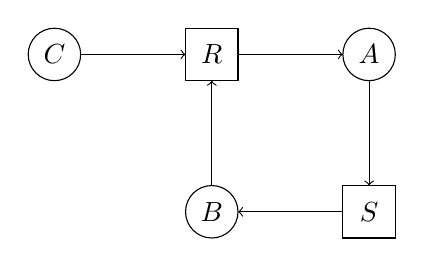
\begin{tikzpicture}[x=0.666cm, y=0.666cm]
                            \begin{scope}[shift={(-3, 0)}]
                                \node at (0.5, -0.5) {$C$};
                                \draw (0.5, -0.5) circle (0.5);
                            \end{scope}
                            \begin{scope}[shift={(0, 0)}]
                                \node at (0.5, -0.5) {$R$};
                                \draw (0, 0) -- (1, 0) -- (1, -1) -- (0, -1) -- cycle;
                            \end{scope}
                            \begin{scope}[shift={(3, 0)}]
                                \node at (0.5, -0.5) {$A$};
                                \draw (0.5, -0.5) circle (0.5);
                            \end{scope}
                            \begin{scope}[shift={(3, -3)}]
                                \node at (0.5, -0.5) {$S$};
                                \draw (0, 0) -- (1, 0) -- (1, -1) -- (0, -1) -- cycle;
                            \end{scope}
                            \begin{scope}[shift={(0, -3)}]
                                \node at (0.5, -0.5) {$B$};
                                \draw (0.5, -0.5) circle (0.5);
                            \end{scope}
                            \draw
                            (-2, -0.5) edge[->] (0, -0.5)
                            (1, -0.5) edge[->] (3, -0.5)
                            (3.5, -1) edge[->] (3.5, -3)
                            (3, -3.5) edge[->] (1, -3.5)
                            (0.5, -3) edge[->] (0.5, -1);
                        \end{tikzpicture}
                    \end{center}
                \item
                    Consider a system that uses the banker's algorithm to avoid deadlocks.
                    At some time a process $P$ requests a resource $R$, but is denied even though $R$ is currently available.
                    Does it mean that if the system allocated $R$ to $P$, the system would deadlock?
                    \medskip

                    No, it is possible for $P$ to complete execution, and free all the resources.
                    However, we no longer have the guarantee that a deadlock will not occur, hence it is \textbf{possible} the system will deadlock.
                \item
                    Two processes $A$ and $B$ each need three records, ~1~, ~2~, and ~3~ in a database.
                    If $A$ asks for them in the order ~1~, ~2~, ~3~, and $B$ asks for them in the same order, deadlock is not possible.
                    However, if $B$ asks for them in the order ~3~, ~2~, ~1~, then deadlock is possible.
                    With three resources, there are $3! = 6$ possible combinations each process can request resources.
                    What fraction of all combinations is guaranteed to be deadlock free?
                    \medskip

                    Since the records are arbitrary, we can reason about it with just one configuration.
                    Assuming $A$ asks for them in ascending order, if $B$ were to also request ~1~ first, one of the two processes would obtain the lock, blocking the other, thus a deadlock will not occur.
                    Therefore, a third of the possible combinations will not result in deadlock.
                \item
                    Can a single-processor system have no processes ready and no process running?
                    Is this a deadlocked system?
                    \medskip

                    Yes, all the processes could be blocked (waiting for I/O) - however typically there is an idle process that runs in this case.
                    This is not a deadlocked system, thus the lack of a running process cannot be used to determine deadlock.
            \end{enumerate}
        \subsection*{Tutorial 6 - Memory Management}
            \begin{enumerate}[1.]
                \itemsep0em
                \item Describe the difference between swapping and paging in the context of virtual memory management.
                    \medskip

                    While both move data from main memory to the disk, swapping moves the entire process's address space into the swap device, whereas paging does this with individual pages from the address space.
                \item What is the advantage of a paged virtual memory system with a
                    \begin{enumerate}[(a)]
                        \itemsep0em
                        \item small page size
                            \medskip

                            There is less unused space, hence less fragmentation.
                        \item large page size
                            \medskip

                            Less overhead, hence translation is faster.
                    \end{enumerate}
                \item What is an associative memory, how does it work, and how is it implemented?
                    \medskip

                    Associative memory is used to cache frequently translated memory addresses.
                    This can be thought of as a table which holds the page number and frame number - instead of checking the page table (in main memory) directly, it can first check if the page number is in this cache, and only accesses the page table when it cannot be found.
                    It is typically implemented in hardware for high performance.
                \item
                    Describe how a context switch affects the virtual memory system.
                    What must the OS do to ensure that memory reference made by the newly-running process will be properly translated?
                    \medskip

                    On a context switch, the page table needs to be changed (the base register in the MMU should be changed to point to the page table in memory), as well as the cache being flushed.
                \item
                    A system implements a paged virtual address space for each process using a one-level page table.
                    The maximum size of an address space is 16 MB.
                    The page table for the running process includes the following entries;
                    \begin{center}
                        \begin{tabular}{|c|c|}
                            \hline
                            page & frame \\
                            \hline
                            0 & 4 \\
                            1 & 8 \\
                            2 & 16 \\
                            3 & 17 \\
                            4 & 9 \\
                            \hline
                        \end{tabular}
                    \end{center}
                    The page size is 1024 bytes, and the maximum physical memory size of the machine is 2 MB.
                    \begin{enumerate}[(a)]
                        \itemsep0em
                        \item How many bits are required for each page table entry?
                            \medskip

                            Since each page is 1 KB, there is a total of $2 \cdot 2^{10} = 2^{11}$ frames on physical memory - this can be represented in 11 bits.
                            By thinking of the page table as an array, each entry needs 11 bits (as well as any additional bits for metadata).
                        \item What is the maximum number of entries in a page table?
                            \medskip

                            Similarly, there can be a total of $16 \cdot 2^{10} = 2^{14}$ pages in the virtual address space.
                        \item How many bits are there in a virtual address?
                            \medskip

                            In a virtual address, there are the 14 bits specifying the page, and then an additional 10, which indicate the offset, thus a total of 24 bits.
                        \item To which physical address will the virtual address 1524 translate to?
                            \medskip

                            Because $1023 < 1524 < 2047$, it lies in page 1.
                            Therefore, it maps to $8 \cdot 1024 + (1524 - 1024) = 8592$.
                        \item Which virtual address will translate to physical address 10020?
                            \medskip

                            Working backwards, it lies in frame 9, hence it is in page 4.
                            Therefore, the virtual address that translates to this is $4 \cdot 1024 + (10020 - 9 \cdot 1024) = 4900$.
                    \end{enumerate}
                \item
                    A pure paging system uses a three level page table.
                    Virtual addresses are decomposed into four fields, $(a, b, c, d)$ with $d$ being the offset.
                    In terms of these constants, what is the maximum number of pages in a virtual address space?
                    \begin{center}
                        $2^{a + b + c}$ pages
                    \end{center}
                \item
                    Calculate the access times for a four-level paging system assuming the following TLB hit ratios. of $80\%$ and $98\%$.
                    Assume that time for memory access is 100ns, and for TLB access 20ns.
                    \begin{enumerate}[(a)]
                        \itemsep0em
                        \item $80\%$
                            $$\underbrace{0.8 \cdot (20 + 100)}_\text{TLB hit} + \underbrace{(1 - 0.8) \cdot (20 + 4 \cdot 100 + 100)}_\text{TLB miss} = 200 \text{ns}$$
                        \item $98\%$
                            $$\underbrace{0.98 \cdot (20 + 100)}_\text{TLB hit} + \underbrace{(1 - 0.98) \cdot (20 + 4 \cdot 100 + 100)}_\text{TLB miss} = 128 \text{ns}$$
                    \end{enumerate}
                    How does this compare to a single-level paging system?
                    \medskip

                    With single level paging, it takes 140ns, and 122ns respectively.
                \item Suppose that pages in a virtual address space a referenced in the following order:
                    \begin{center}
                        ~1 2 1 3 2 1 4 3 1 1 2 4 1 5 6 2 1~
                    \end{center}
                    There are three empty frames available.
                    Assume that paging decisions are made on demand (when page faults occur).
                    Show the contents of the frames after each memory reference, and the number of page faults;
                    \begin{enumerate}[(a)]
                        \itemsep0em
                        \item the LRU replacement policy \hfill 11 faults
                            \begin{center}
                                \begin{tabular}{l|ccccccccccccccccc}
                                    \multirow{2}{*}{frame} & \multicolumn{17}{c}{reference} \\
                                    & 1 & 2 & 1 & 3 & 2 & 1 & 4 & 3 & 1 & 1 & 2 & 4 & 1 & 5 & 6 & 2 &  1 \\
                                    \hline
                                    0 & 1 & 1 & 1 & 1 & 1 & 1 & 1 & 1 & 1 & 1 & 1 & 1 & 1 & 1 & 1 & 2 & 2 \\
                                    1 &   & 2 & 2 & 2 & 2 & 2 & 2 & 3 & 3 & 3 & 3 & 4 & 4 & 4 & 6 & 6 & 6 \\
                                    2 &   &   &   & 3 & 3 & 3 & 4 & 4 & 4 & 4 & 2 & 2 & 2 & 5 & 5 & 5 & 1 \\
                                    fault & $\times$ & $\times$ & & $\times$ & & & $\times$ & $\times$ & & & $\times$ & $\times$ & & $\times$ & $\times$ & $\times$ & $\times$
                                \end{tabular}
                            \end{center}
                        \item the clock policy \hfill 9 faults
                            \begin{center}
                                \begin{tabular}{l|ccccccccccccccccc}
                                    \multirow{2}{*}{frame} & \multicolumn{17}{c}{reference} \\
                                    & 1 & 2 & 1 & 3 & 2 & 1 & 4 & 3 & 1 & 1 & 2 & 4 & 1 & 5 & 6 & 2 &  1 \\
                                    \hline
                                    0 & 1 & 1 & 1 & 1 & 1 & 1 & 4 & 4 & 4 & 4 & 4 & 4 & 4 & 5 & 5 & 5 & 5 \\
                                    1 &   & 2 & 2 & 2 & 2 & 2 & 2 & 2 & 1 & 1 & 1 & 1 & 1 & 1 & 6 & 6 & 6 \\
                                    2 &   &   &   & 3 & 3 & 3 & 3 & 3 & 3 & 3 & 2 & 2 & 2 & 2 & 2 & 2 & 1 \\
                                    fault & $\times$ & $\times$ & & $\times$ & $\times$ & & $\times$ & & $\times$ & & $\times$ & & & $\times$ & $\times$ & &
                                \end{tabular}
                            \end{center}
                    \end{enumerate}
            \end{enumerate}
        \subsection*{Tutorial 7 - Device Management}
            \begin{enumerate}[1.]
                \itemsep0em
                \item 
            \end{enumerate}
        \subsection*{Tutorial 8 - Disk Management}
            \begin{enumerate}[1.]
                \itemsep0em
                \item 
            \end{enumerate}
        \subsection*{Tutorial 9 - File Systems}
            \begin{enumerate}[1.]
                \itemsep0em
                \item 
            \end{enumerate}
        \subsection*{Tutorial 10 - Security}
            \begin{enumerate}[1.]
                \itemsep0em
                \item 
            \end{enumerate}
\end{document}